\documentclass[journal]{IEEEtran}

\usepackage[utf8]{inputenc}
\usepackage[T1]{fontenc}
\usepackage{silence}\WarningsOff[latexfont]

\usepackage{amsmath}

\RequirePackage{tikz}[2010/10/13]
\usetikzlibrary{arrows,automata,calc,intersections,patterns,decorations.pathmorphing,decorations.pathreplacing}

\usepackage{graphicx}
\usepackage{cite}
\usepackage{url}
\usepackage[caption=false,font=footnotesize]{subfig}
\usepackage[binary-units,per-mode=symbol]{siunitx}
\sisetup{list-final-separator = {, and }}
\usepackage{booktabs}
\usepackage{pifont}
\usepackage{microtype}
\usepackage{textcomp}
\usepackage[american]{babel}
\usepackage[noabbrev,capitalise]{cleveref}
\usepackage{xspace}
\usepackage{hyphenat}
\usepackage[draft,inline,nomargin,index]{fixme}
\fxsetup{theme=color}
\usepackage{grffile}
\usepackage{xfrac}
\usepackage{multirow}
\RequirePackage{xstring}
\RequirePackage{xparse}
\RequirePackage[index=true]{acro}
\NewDocumentCommand\acrodef{mO{#1}mG{}}{\DeclareAcronym{#1}{short={#2}, long={#3}, #4}}
\NewDocumentCommand\acused{m}{\acuse{#1}}
\usepackage{upquote}
\usepackage{systeme}
\usepackage{dblfloatfix}
\usepackage{listings}

\graphicspath{ {./images/} }

% Keywords command
\providecommand{\keywords}[1]
{
	\small	
	\textbf{\textit{Keywords---}} #1
}


\begin{document}
\title{MQTT Bandwidth Estimation\\ in a Docker Virtual Environment}

\author{
	\IEEEauthorblockN{Simone Bernabè, Mat. number 207485\\}
	\texttt{simone.bernabe@studenti.unitn.it}
}

\makeatletter
\def\endthebibliography{%
	\def\@noitemerr{\@latex@warning{Empty `thebibliography' environment}}%
	\endlist
}
\makeatother

\markboth{MQTT Protocol - Project Course 2020}{}

\maketitle

\begin{abstract}
MQTT is an essential and growing protocol, engineered for IoT (Internet of Things) and designed to preserve power \cite{lowp}, to works well on unreliable networks, and to be a light but a secure protocol. The following document is an extensive benchmark and test on MQTT bandwidth over some typical usage and different configurations. The objective is estimating the protocol minimum bandwidth request between sensors (\textbf{publishers}) and broker, and between broker and applications (\textbf{subscribers}). Tests was led using modern technology, creating a virtual network with the usage of Docker's container acting as sensors, and a broker, implemented with Eclipse Mosquitto \cite{mosquitto}. All the results have then been resumed with plots, raw data and simple formulas to compute a bandwidth consumption estimation.
\end{abstract}
\hspace{10pt}

%TC:ignore
\keywords{mqtt, bandwidth, docker}

\acresetall

\section{Introduction}
\label{sec:introduction}
MQTT is a lightweight protocol that transports messages between devices, and it is today widely used in the field of "Internet of Things (IoT) \cite{mqtt}". 
It's clear how this protocol represents right now state of the art for that type of connection and for a lot of other uses, where publish and subscribe paradigm comes advantageous. Still, there are no much documentation and tests on how much scalable the protocol is with different types of implementation and which is the minimum bandwidth request with a high number of communicating elements in place. This work aims to characterize the traffic generated by this protocol in different configurations, both between sensors and broker, that between broker and applications. The protocol has therefore been tested with different numbers of sensors and sinks configuration, which placed before sensors, allow to convoy and parse the traffic more efficiently. Besides this, the sensors use multiple messages propagation probability distribution. 

A peculiarity of this test is the environment in which has been tested. As a matter of fact, the test has been conducted in a virtual network created using Docker container and a virtual machines, allowing to easily scale the network size. The generated message was finally captured and analysed using the Wireshark application and iftop command \footnote{http://www.ex-parrot.com/pdw/iftop/}. 

The document also gives a detailed insight on MQTT protocol, in all the mechanics of functioning and all the possible optimization that can be enforced to enhance the bandwidth consumption. 

In the following chapters, there are an introduction to the MQTT protocol structure as well as the functioning, 
The rest of the paper is organized as follows: Section 2 introduces the MQTT protocol, 
describing the structure and functioning,
Section 3 describes the process of preparations of the bench, which has then
been used in Section 4. Section 5 draws the Conclusions.

\section{MQTT Protocol}
MQ Telemetry Transport (MQTT) is a lightweight broker-based publish/subscribe messaging protocol designed to be open, lightweight, and easy to implement. It was designed as an extremely lightweight protocol to allow the application in remote locations with a limited internet connection and small low power devices. These principles also turn out to make the protocol ideal of the emerging "machine-to-machine" (M2M) or "Internet of Things" world of connected devices, and for mobile applications. 

The protocol was first invented by IBM in 1999 and has now become an OASIS/ISO standard with the latest release version \cite{mqtt_spec}.

The protocol runs over TCP/IP and typically on port 1883, which is assigned by the Internet Assigned Numbers Authority (IANA). For using MQTT over SSL, port 8883 is used. 

In image \ref{fig:flow} there is a communication example, with a sensor publishing temperature over a topic and a client subscribed to that topic receiving it. 
A Packet consists of up to three parts, always in the following order, as shown below in figure \ref{fig:packet}.

\begin{figure}[h]
	\centering
	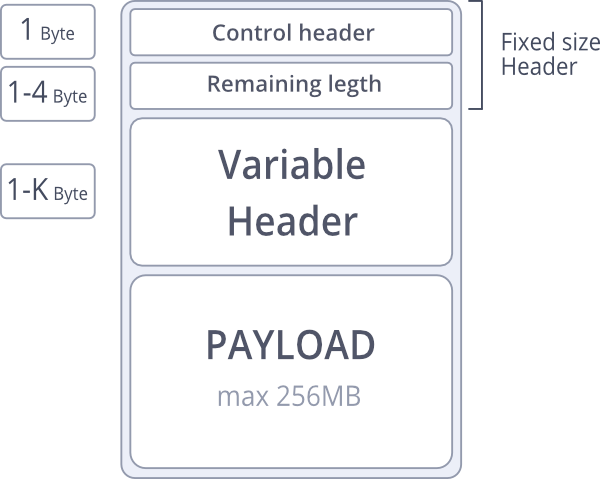
\includegraphics[width=0.35\textwidth]{mqtt_2}    
	\caption{MQTT packet format, with fixed header, variable header and payload}
	\label{fig:packet}
\end{figure}

\subsection{Fixed header}
This header is present and mandatory in all the packet types, and contain the Control field that is divided in protocol commands, message type field, and control flags \cite{steven}.
Control flags include the \textbf{QoS} (Quality of Service) selection, to ensure the reliability of messaging \cite{qoslevel}.
Figure \ref{fig:qos_level} shows the three different version of QoS, and later on the paper, there will be a focus on the overhead caused by the QoS levels. 

\begin{figure}[h]
	\centering
	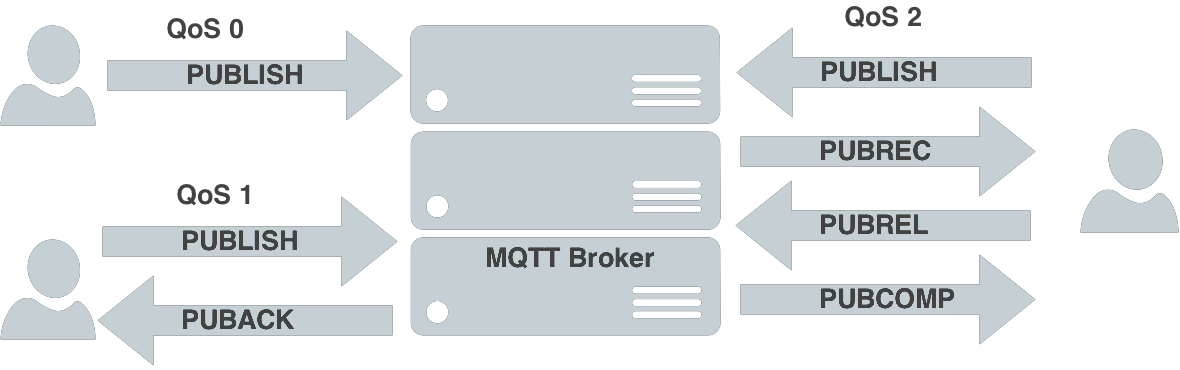
\includegraphics[width=0.46\textwidth]{qos_str}    
	\caption{QoS levels packet exchange}
	\label{fig:qos_level}
\end{figure}

The second part (starting from Byte 2) is instead the Remaining Length, a Variable Byte Integer that represents the number of bytes remaining within the current Control Packet, including data in the Variable Header and the Payload.

\subsection{Variable header}
Some types of MQTT Control Packets contain a Variable Header component. It resides between the Fixed Header and the Payload. 
The content of the Variable Header varies depending on the packet message type. 
For example, the publish message includes a \textbf{topic} field, which refers to the argument or directory (\textbf{topic}) in which the client publishes its messages. This field has a maximum size of 65536 Byte. 

\subsection{Payload}
The last part is nothing less than the message the client wants to send. The maximum size of 256MB is limited by the 4 Byte of the Remaining length field I mentioned before. 
\begin{figure}[h]
	\centering
	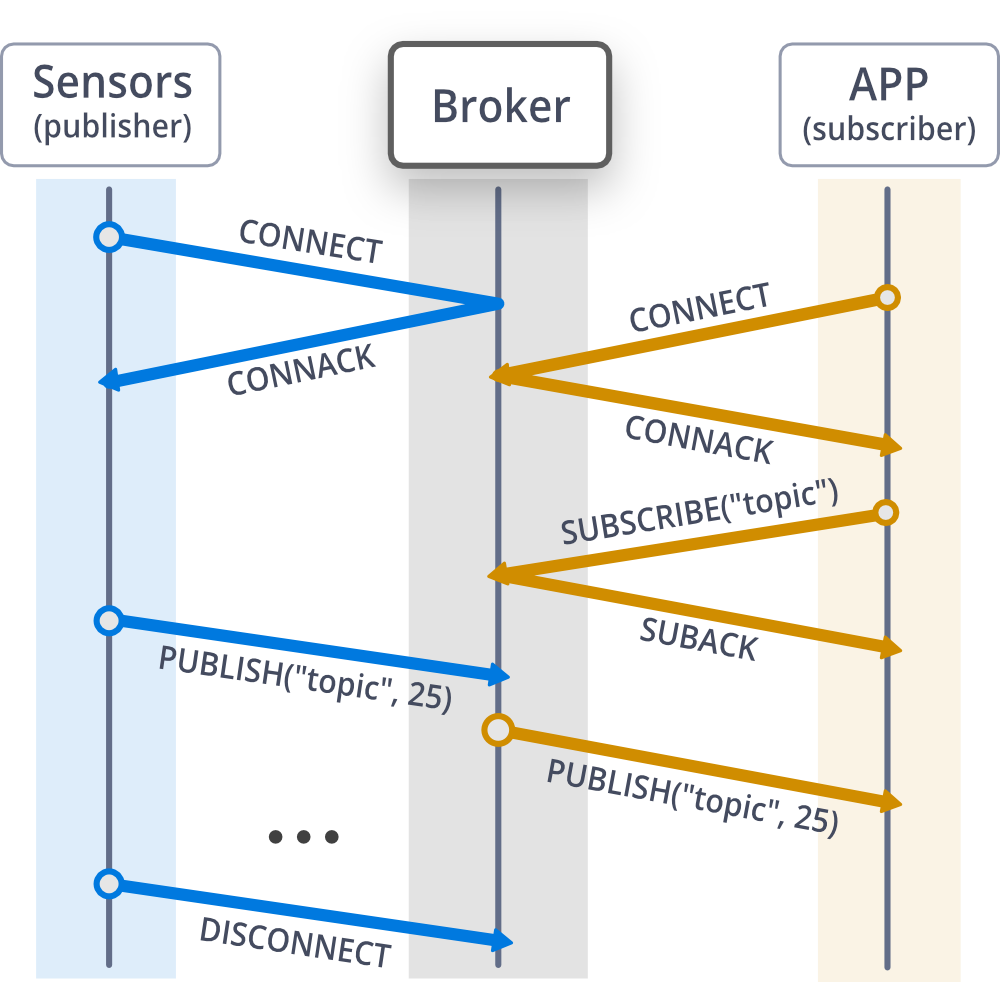
\includegraphics[width=0.4\textwidth]{mqtt}
	\caption{MQTT communication: A sensors connect to the broker and \text{publish} to a topic some value. Meanwhile, an app has connected to the broker and \textbf{subscribe} to the same topic. So, the broker forwards the message published by the sensor to the app.}
	\label{fig:flow}
\end{figure}

\section{Preparation}
To complete the bandwidth tests, I tried multiple configurations, and with it, I found issues and tricky situation that I'll explain later on. 
The final architecture that is shown in figure \ref{fig:strut}, has $N$ sensors based on docker container and an MQTT broker on a virtual machine. The application side (subscribers) has been simulated using MQTT.x, a simple client that allows to visualize and subscribe to a broker directly. 
\begin{figure}[h]
	\centering
	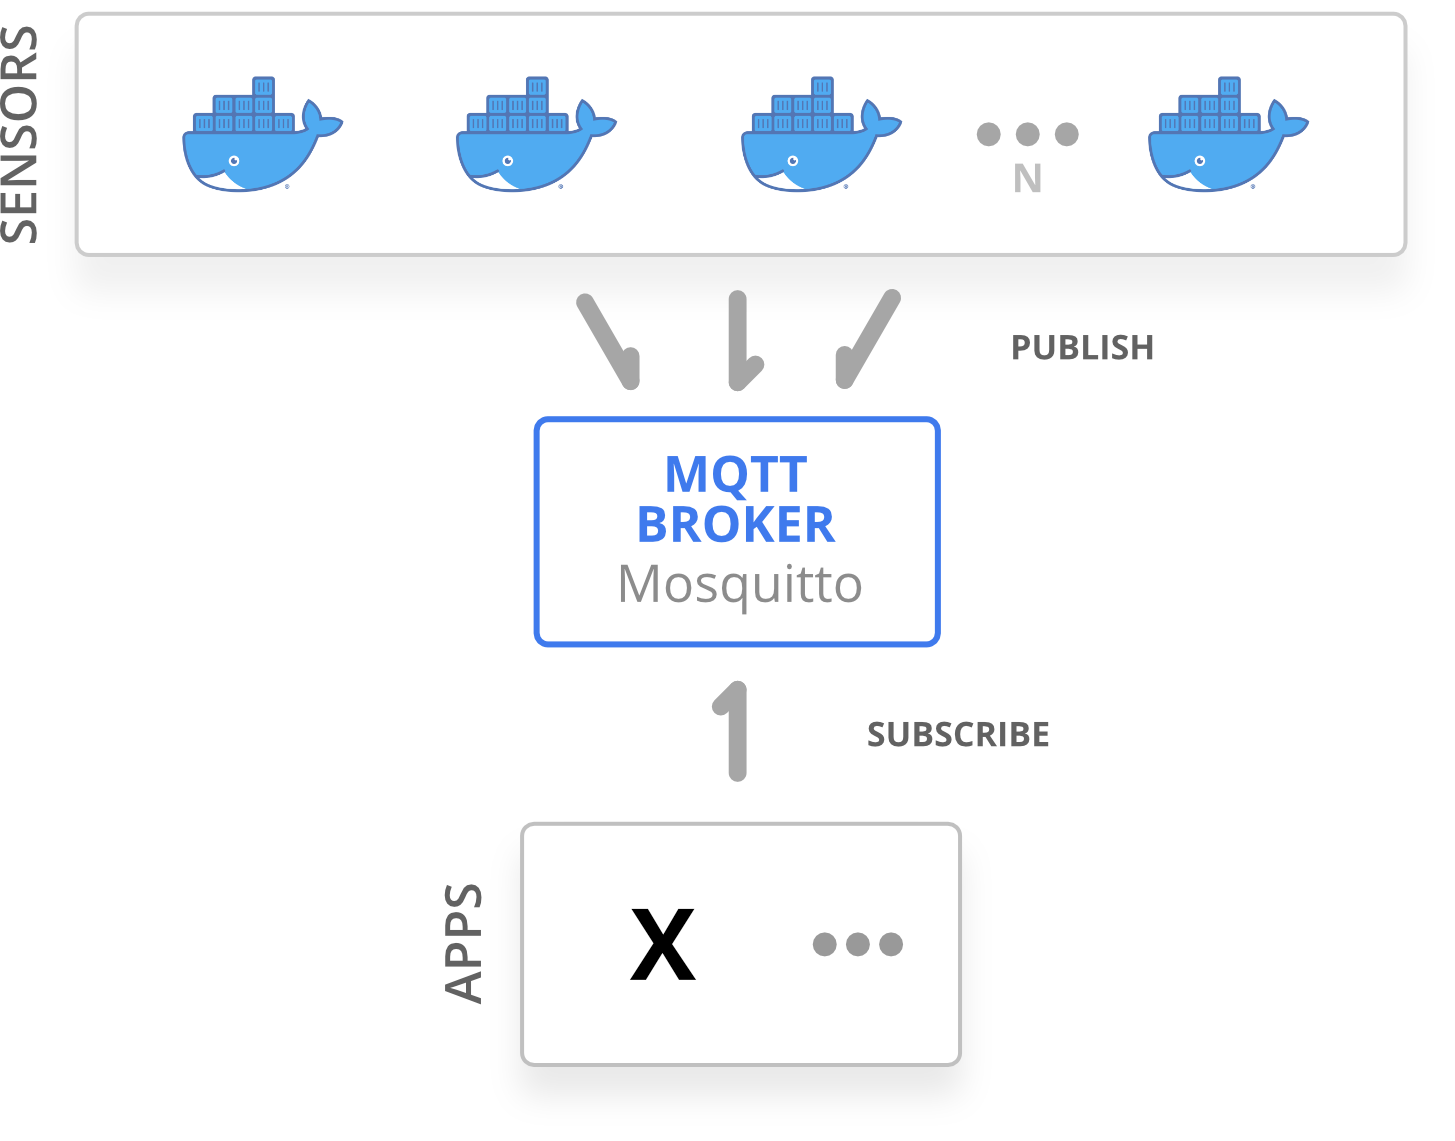
\includegraphics[width=0.45\textwidth]{struttura}
	\caption{Testing architecture}
	\label{fig:strut}
\end{figure}

\subsection{Docker Sensors (publisher)}
\label{sec:sensors}
To simulate the sensor (publisher), I choose a minimal docker container based on Alpine Linux distribution, and I use docker-compose tool to organize and manage the start-up of the environment. 
A virtual network like this allows you to conveniently scale on the number of sensors and devices in use.

Each container should then publish information to a given topic. An initial try was to use a simple bash script to publish on broker using the Mosquitto client commands. Unfortunately, that command does not manage sessions and every message from a client is independent one another and every exchange represent a new session. Consequently, every communication includes a connection and a disconnection message, creating an overhead due to an unnecessary exchange of control messages.

A library and a programming language are needed to take advantages of MQTT protocol completely and thus to optimize the communication. I choose C after trying several others, because of its lightness and integration. 
Python requires too many disk space resources and is slower, while Java is too heavy since it is running on its JVM (20MB RAM occupation). 
C implementation is a little more tricky, but it does not need any installation on the container and the RAM occupation once running has set to an incredible 0.9MB. Simulating 100 sensors take only 90MB of RAM occupation, and this gives me also more flexibility on testing. 

The final program consists of three modalities: 

\begin{itemize}
	\item \textbf{\{n\} sec delay}: Sensors send a publish message on a given topic every {n} seconds. This way, all the sensors have the same behaviour, and since they are practically concurrent, they produce a heavy load on the bandwidth. 
	\item \textbf{Realistic}: This instead randomize the sending behaviour, offsetting all the sensor and creating a more realistic behaviour, close to an implementation where sensor responds to events. 
	\item \textbf{\{N\} Random payload}: Every sensor sends a message with a specified sized payload
\end{itemize}

To manage all this configurations the container executable takes four optional parameters:

\begin{center}
	./publish \{method\} \{sink\} \{n sensors/sinks\} \{payload size\}
\end{center}

\textbf{Sinks} on the other hand, is based on the same container image, but takes different parameters in the executable. A sink is simulated grouping MQTT messages, as it has been sent from $N$ sensors and then routed through one. TCP packet containing more than one MQTT message drastically reducing the header overhead caused by the protocol stack. Figure \ref{fig:overhead} shows exactly the structure difference between usual sensors publish message versus sinks one. 

\begin{figure}[h]
	\centering
	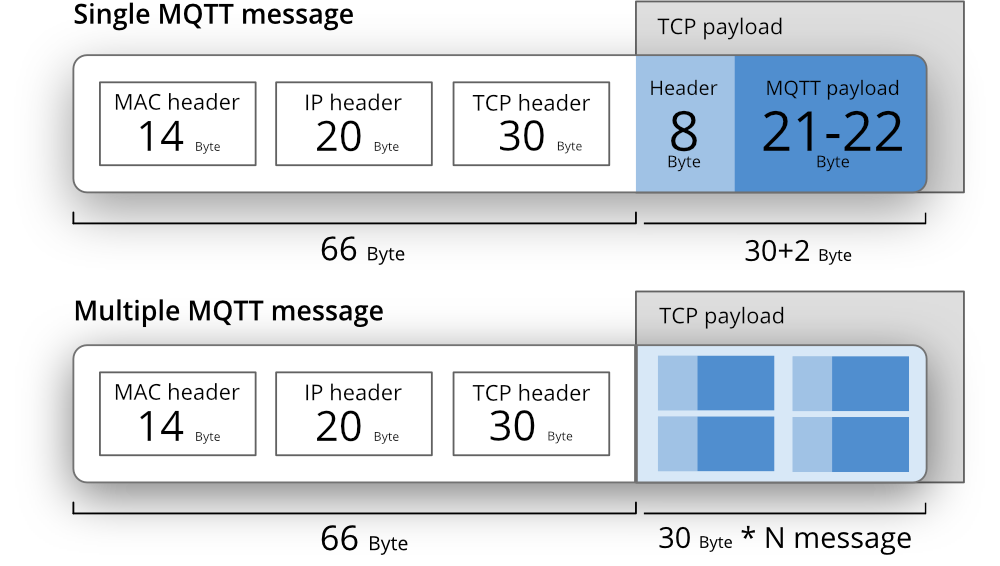
\includegraphics[width=0.48\textwidth]{mqtt_3}
	\caption{Overhead of the protocol aside the specific MQTT message used in this tests. Second image represent a MQTT grouping of message}
	\label{fig:overhead}
\end{figure}

An example of a command to launch 1 sink and 10 sensors using the docker-compose command: 

\begin{lstlisting}[language=bash, caption={Docker-compose launch command}]
docker-compose up -scale client=10 -scale sink=1
\end{lstlisting}

\subsection{Broker}
Broker is based on Eclipse mosquitto release \cite{mosquitto}, that is currently one of the most used implementations. 
An official docker image exists for mosquitto that work just fine out of the box. 
For convenience, Mosquitto has been installed on a minimal Alpine virtual machine to better sniff on the network interface using Wireshark application and iftop appliance. 

\subsection{Applicazione (subscriber)}
On the other side, the subscriber was simulated using an interface called MQTT.x that allow to easily subscribe to multiple topics and see the incoming message, also the one related to the connection. 

\section{Testing}
This chapter finally analyses the result of all the tests taken and present a simple formula that estimates bandwidth according to the payload, Qos level and numbers of sensors. 
Bench configuration: 
\begin{itemize}
	\item Testing message published by the sensors: "\{N\} C° - Humidity: \{K\}\% " with K > 10. This way the payload is in range 21-22 Byte. Figure \ref{fig:overhead} shows exactly this values with all the other overhead. 
	\item 200 seconds sample to measure bandwidth using both iftop and Wireshark. 
	\item Besides the test on QoS, all the other tests were executed using QoS 0. 
\end{itemize}

\subsection{Sensors number bandwidth analysis}
Figure \ref{fig:sensors} shows the correlation between number of sensors publishing and bandwidth request (KByte/s). The plot is represented using a logarithmic scale. The lines show the different type of propagation, as explained above in section \ref{sec:sensors}. Docker light implementation allows me to scale the sensors network up to 500+ elements easily.

\begin{figure}[h]
	\centering
	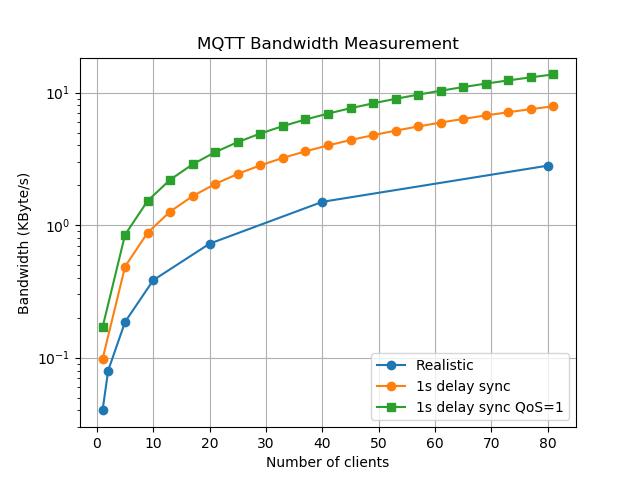
\includegraphics[width=0.50\textwidth]{sensors}
	\caption{MQTT bandwidth with different propagation profile and sensors number}
	\label{fig:sensors}
\end{figure}

With the relatively small payload considered, the results were nearly linear since no congestion or packet division came in. 

\subsection{Bandwidth analysis introducing sinks}
Figure \ref{fig:sinks}, instead, shows what happens when a sink is introduced, aggregating and routing packets. Sinks allow creating a single TCP packet with multiple MQTT messages inside, drastically reducing the overhead of the IP protocol stack. In the plot, as we can see, the bandwidth generated by 400+ sensors publishing and passing through a sink is less than half as if they had been sent individually.
\begin{figure}[h]
	\centering
	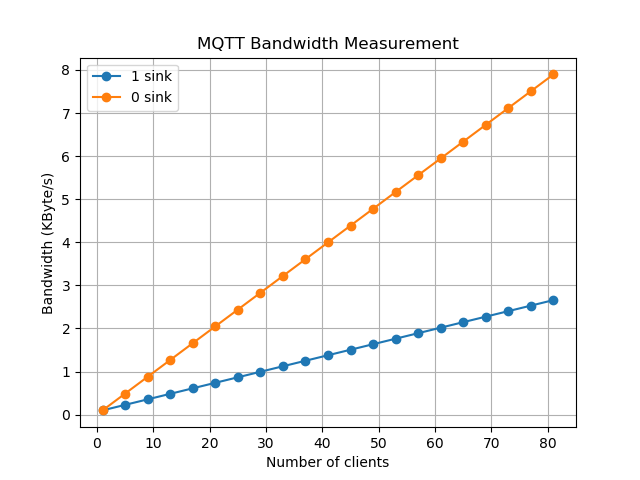
\includegraphics[width=0.50\textwidth]{sinks}
	\caption{Bandwidth comparison with the introduction of a sink}
	\label{fig:sinks}
\end{figure}

\subsection{Bandwidth analysis with different QoS levels}
Referring to the already seen figure \ref{fig:qos_level} we can see in Figure \ref{fig:qos} how much the reliability of messaging costs in term of bandwidth. Level 0 sends the message only once following the message
distribution flow and does not check whether the message
arrived at its destination. Level 1 (at least once) check the delivery with a PUBACK. If PUBACK is lost, the same message could be sent two times. Level 2 overcome this having 4-way handshake, needing a lot more bit to process the message. 

Important to notice that TCP ACK differs from MQTT ACK. In QoS 0, every MQTT publishes are followed by a TCP ACK. In QoS 1 a publish message get both a TCP network standard ACK and a PUBACK that is instead related to MQTT protocol. 

\begin{figure}[h]
	\centering
	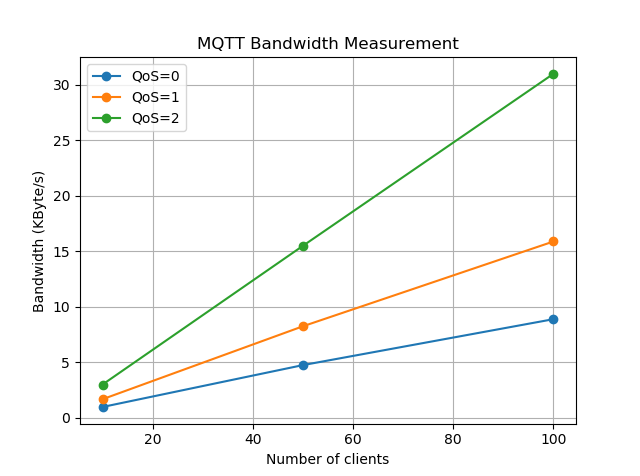
\includegraphics[width=0.50\textwidth]{qos}
	\caption{QoS total bandwidth comparison}
	\label{fig:qos}
\end{figure}

Figure \ref{fig:loss} show rather how QoS impact also on message loss, in particular on a wireless network where there are a lot more packet loss \cite{qoslevel}. 
The data consumption reduces to about 50\% on using QoS 1 from QoS 2. Similarly, QoS 0 uses 40\% less data than QoS1 \cite{datausage}.

\begin{figure}[h]
	\centering
	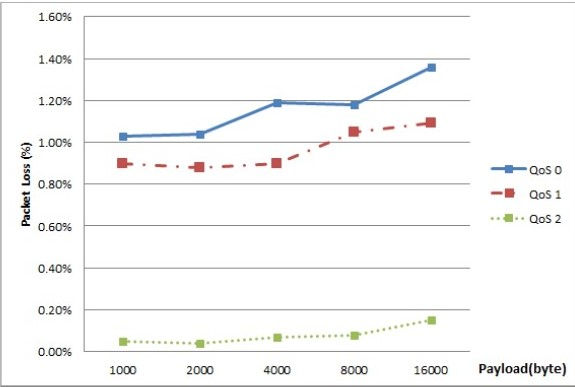
\includegraphics[width=0.40\textwidth]{loss}
	\caption{Wireless Network message loss analysis result by Keimyung University \cite{qoslevel}}
	\label{fig:loss}
\end{figure}

\subsection{Bandwidth analysis with different payload size}
The last test was probably the more significant and is based on payload size and how the overhead caused by transport protocol and MQTT QoS impact on total publish messages flow. In particular, a factor to analyze is the overhead caused by the packet division that occurs when frames reach and exceed the 1460 Byte frame limit, known as MSS (Maximum Segment Size). For example 4kB (4,000 Bytes) must be split into 3 packets, each packet not exceeding 1460 Bytes (4,000 / 1460 = 2,739). 
3 x 50 Bytes of TCP and IP headers equals a 150Byte, so around 3\% of TCP/IP overhead
Thus, 4,150Btyes of data is transmitted over the network. 
A percentage that becomes relatively smaller the more the payload size, but that has a significant impact with a smaller packet. 

Figure \ref{fig:payload} show exactly the impact of the QoS and TCP segmentation overhead on packets with different payload size. It's visible as, after the payload exceeds the maximum segment size of 1460Byte, the overhead starts to grow. This behavior has been registered only on QoS 1 and QoS 2, where other MQTT packet (PUBACK, PUBREL, PUBCOMP) is present. In QoS 0 the segment gets the ACK always at the end of segments transmission, one time, so the overhead is constant. 

\begin{figure}[h]
	\centering
	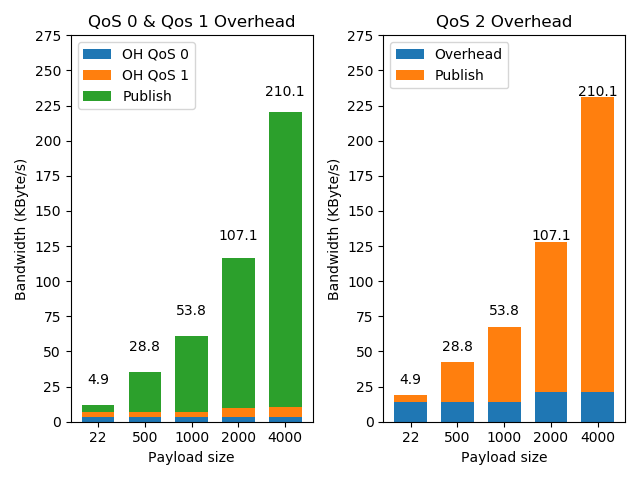
\includegraphics[width=0.50\textwidth]{payload}
	\caption{Overhead of the protocol QoS on different Payload size}
	\label{fig:payload}
\end{figure}

\subsection{Correlations}
Based on the results above, I created a formula to estimate the bandwidth generated given all the configuration.
I define a pseudo-constant header overhead parameter $H_c$  that is the sum of the size of the headers from Layer 1, 2 and 3
that are present in every sent packet. 
\begin{equation}
H_c = H_{mac} + H_{tcp} + H_{ip} = 14 + 20 + 32 = 66 Byte
\end{equation}\\
Then I define the formula to compute MQTT message based on the payload size ($P$). In this case, only publish message is considered.
\begin{equation}
M_P = 1 + L + VH + P 
\end{equation}\\
where $L \in [1,4]$ and $VH \in [1, n] $ depending on payload size and message type.

Finally the bandwidth estimation based on QoS 0:
\begin{equation}
B_E (P, pps, N_s) = (M_P + H) * N_s * pps
\end{equation}\\
where $P$ is the payload size, $pps$ is the packet per second rate and $N_s$ is the number of sensors publishing message. 

With other QoS, the algorithm needs to take into account the overhead of PUBACK, PUBREL and PUBCOMP. 

With the parameter used in these tests, the size of the MQTT packet is showed in Figure \ref{fig:overhead}, as well as PPS that is 1 packet/s with 1s configurations.  

\section{Conclusions}
This document has presented a deep test on MQTT protocol using a peculiar virtual network, using Docker, allowing to scale on great number of sensors. All the analysis show the correlation and the association of bandwidth with other tests parameters configuration. In particular, the impact of QoS (Quality of Service) on the number of packets sent per transmission, and consequently on band request.

All the parameters have been synthesized in a convenient formula that roughly estimates the MQTT bandwidth request. 

Working on this tests, I reach significant number, in terms of clients and payload. Considering the real purpose of MQTT protocol, this number are unlikely in most of its implementation, but they can outline an upper bound. Bandwidth request though is noticeably restrained, compared with competitor protocol, on ideal packet payload. 

In conclusion, the analysis that can be carried on a virtual network like this are limitless; in particular, this implementation is already ready to go for future works \footnote{https://github.com/simoberny/mqtt-docker-bench}.

\bibliographystyle{IEEEtran}
\bibliography{references}

\end{document}
